% !TEX TS-program = pdflatex
% !TEX encoding = UTF-8 Unicode

% This is a simple template for a LaTeX document using the "article" class.
% See "book", "report", "letter" for other types of document.

\documentclass[12pt]{article} % use larger type; default would be 10pt

\usepackage[utf8]{inputenc} % set input encoding (not needed with XeLaTeX)
\usepackage[danish]{babel}

%%% Examples of Article customizations
% These packages are optional, depending whether you want the features they provide.
% See the LaTeX Companion or other references for full information.

%%% PAGE DIMENSIONS
\usepackage{geometry} % to change the page dimensions
\geometry{a4paper} % or letterpaper (US) or a5paper or....
% \geometry{margin=2in} % for example, change the margins to 2 inches all round
% \geometry{landscape} % set up the page for landscape
%   read geometry.pdf for detailed page layout information

\usepackage{graphicx} % support the \includegraphics command and options

% \usepackage[parfill]{parskip} % Activate to begin paragraphs with an empty line rather than an indent

%%% PACKAGES
\usepackage{setspace}
\usepackage{booktabs} % for much better looking tables
\usepackage{array} % for better arrays (eg matrices) in maths
\usepackage{paralist} % very flexible & customisable lists (eg. enumerate/itemize, etc.)
\usepackage{verbatim} % adds environment for commenting out blocks of text & for better verbatim
\usepackage{subfig} % make it possible to include more than one captioned figure/table in a single float
\usepackage{enumitem}
% These packages are all incorporated in the memoir class to one degree or another...

%%% HEADERS & FOOTERS
\usepackage{fancyhdr} % This should be set AFTER setting up the page geometry
\pagestyle{fancy} % options: empty , plain , fancy
\renewcommand{\headrulewidth}{1pt} % customise the layout...
\lhead{}\chead{}\rhead{}
\lfoot{}\cfoot{\thepage}\rfoot{}

%%% SECTION TITLE APPEARANCE
\usepackage{sectsty}
\allsectionsfont{\sffamily\mdseries\upshape} % (See the fntguide.pdf for font help)
% (This matches ConTeXt defaults)

%%% ToC (table of contents) APPEARANCE
\usepackage[nottoc,notlof,notlot]{tocbibind} % Put the bibliography in the ToC
\usepackage[titles,subfigure]{tocloft} % Alter the style of the Table of Contents
\renewcommand{\cftsecfont}{\rmfamily\mdseries\upshape}
\renewcommand{\cftsecpagefont}{\rmfamily\mdseries\upshape} % No bold!

\usepackage[scaled]{helvet}
\renewcommand\familydefault{\sfdefault} 
\usepackage[T1]{fontenc}

%%% END Article customizations

%%% The "real" document content comes below...

\begin{document}
\onehalfspacing
\begin{titlepage}
	\centering
	
\includegraphics[width=0.3\textwidth]{ucllogo}\par\vspace{1cm}
	{\scshape\LARGE UCL Erhvervsakademi og Professionshøjskole \par}
	\vspace{1cm}
	{\scshape\Large Synopsis\par}
	\vspace{1.5cm}
	{\huge\bfseries .NET Core og Microservices \\ \large Koordinering af forretningsprocesser på tværs af services\par}
	\vspace{2cm}
	{\Large\itshape Julian Mathias Kock\par}
	\vfill
	Underviser \par
	~Kaj \textsc{Bromose}
	\vfill
% Bottom of the page
	{\large \today\par}

\end{titlepage}

\tableofcontents
\newpage

\section{ Indledning }
Vores verden er blevet en digital verden. Alt lige fra ens køleskab og elkedler til valutaer og telefoner er blevet digitale. Internetforbindelserne bevæger sig nu med lysetshastighed og en efterspørgelse på ingen nedetid, hurtige svartider og overskuelighed er blevet hverdag for udviklere. 
\newline

\noindent
Softwaren der udvikles har aldrig været under så stort et pres. Udviklere bliver sat til at løse endnu mere komplekse forretningsprocesser hvor hver enkelt kodeblok skal være let læselig, skalerbart og omskiftelig. Samtidig skal koden være gennemtestet, virke i alle mulige forskellige miljøer og integrere let mod andet software. 
\newline

\noindent
Med andre ord er arkitekturen samt infrastrukturen blevet vigtigere end aldrig før. For at imødekomme alle disse krav har man kigget mod opdeling af kode i en service baseret arkitektur, hvor hver service tildeles et ansvar og kan blive udviklet og skaleret individuelt. Fokus i dette fag har været Microservices som er et term for mange autonome services der arbejder sammen for at udarbejde og give en forretningsmæssigværdi\cite{newman2015building}.
\newline

\noindent
Denne opgave vil fokusere på den koordinering der skal til for at Microservices kan løse forretningsmæssigeopgaver, samtidig med at services skal være autonome og opnå eventual consistency.
\newline

\newpage
\section{ Problemformulering }

\textbf{Hvordan opnår man en fornuftig koordinering af Microservices til at løse forretningsmæssigeopgaver?}
\newline

\noindent
Del spørgsmål

\begin{itemize}
  \item[1] Hvad er SAGA-mønstret?
  \item[2] Hvordan kan man sikre autonome Microservices?
  \item[3] Hvad skal din Microservices tage højde for at opnå eventual consistency?
\end{itemize}

\section{ 1. delspørgsmål }
\subsection{ Saga pattern }
Når der tales om koordineringen af Microservices menes der den interne kommunikation/dataudveksling der skal til for at services kan udføre en forretningsproces. Et eksempel på en forretningsproces kunne f.eks. være at lave en ordre der tilsidst afsendes og modtages af en kunde. I en traditionel arkitektur kunne man bruge ACID transaktioner, men når der er tale om flere services er det svært at lave isoleret transaktioner. En måde hvorpå man kan imødekomme dette er ved brug af distrubureret transaktioner, så som 2PC (two-phase commit). Denne løsning kan være tilstrækkelig, men den giver dog nogle ekstra problemer. Ideén med distrubureret transaktioner er at alle services der indgår enten committer transaktioner eller laver en rollback. Det betyder altså at du nu er direkte afhængig af, om alle services er klar til og modtage requestet, eller ej. Derfor vil negativ downtime for en service have effekt på alle andre services der indgår i den distribureret transaktion\cite{richardson2019microservices}. Dette bryder på autonom princippet bag Microservices, og der er nu en direkte afhængighed videre fra service til service.
\newline

\noindent
For at imødekomme kommunikation der skal gå på tværs af services kan man her bruge et Saga pattern. Saga mønstret er et mønstre hvorpå man kan lave transaktioner på tværs af services. Der findes to typer af sager. Choreography baseret og orchestration baseret\cite{richardson2019microservices}.

\subsection{ Orchestration saga }

\begin{figure}[h]
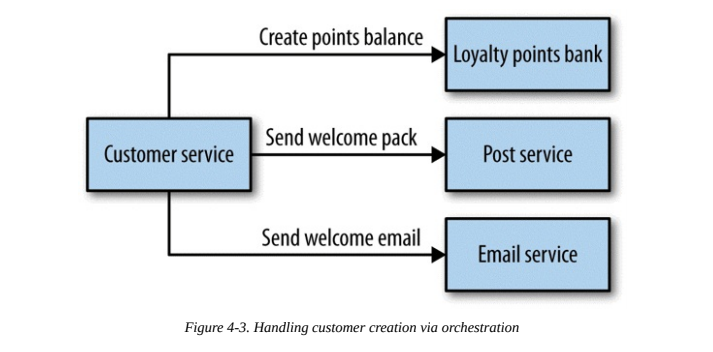
\includegraphics[width=1\textwidth]{orchestrationsaga}
  \caption{\cite[p.~91]{newman2015building}}
\end{figure}

\noindent
For at forstå orchestration bruges oftest en analogi til den virkelige verden hvor man kigger på et orkester. I et orkester er der en person der orkestrerer orkestret, nemlig dirigenten. Dirigenten sørger for at alle i orkesteret rammer deres toner på de rigtige tidspunkt og aggregere alle instrumenters toner til at få leveret et stykke musik. Med denne analogi kan vi kigge på services som de enkelte instrumenter, og dirigenten som en Saga der sørger for at aggregere og præsentere data fra forskellige services. Et simpel eksempel kunne være en request/response hvor en klient beder om at få alle informationer om en kunde og kundens betalinger baseret på kundens id. Saga'en vil requeste kundeservicen der kan returnere detaljer om kunden og requeste betalingsservicen om alle betalinger oprettet af kunden. Saga'en vil så aggregere dette data og præsentere det i et response. En definition på en orkesteringssaga kunne være følgende.
\newline

\emph{Orchestration saga} - I en orkesterings baseret saga centraliserer man koordinations logikken i en enkelt service. Denne service står for at sende beskeder afsted til services der fortæller dem hvilke funktioner de skal udføre og eventuelt aggregere data til et response\cite{richardson2019microservices}.

\subsection { Choreography saga }
\begin{figure}[h]
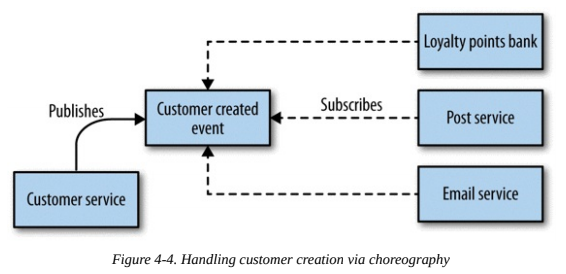
\includegraphics[width=1\textwidth]{cheographysaga}
  \caption{\cite[p.~92]{newman2015building}}

\end{figure}
\section { 2. delspørgsmål }
\subsection { Consumer-Driven Contracts }
\section { 3. delspørgsmål }
\subsection { Hvad er eventual consistency? }
\subsection { Hvordan tager man højde for eventual consistency? }


\newpage
\bibliographystyle{plain}
\bibliography{bibliography}
\end{document}

